% =====================================================================
%  The Factor Model Cookbook
%  The whole workflow, written as recipes, as if you did it by hand
%
%  Build:  pdflatex -interaction=nonstopmode factor-model-cookbook.tex  (twice)
% =====================================================================
\documentclass[11pt,a4paper]{article}

\usepackage[T1]{fontenc}
\usepackage[utf8]{inputenc}
\usepackage[english]{babel}
\usepackage{lmodern}
\usepackage{mathpazo}
\usepackage[scaled=0.90]{helvet}
\usepackage{microtype}
\usepackage[a4paper,top=28mm,bottom=26mm,left=30mm,right=30mm,headheight=22pt]{geometry}
\usepackage{amsmath,amssymb}
\usepackage[most]{tcolorbox}
\usepackage{booktabs,array,longtable,tabularx}
\usepackage{xcolor}
\usepackage{titlesec}
\usepackage{fancyhdr}
\usepackage{enumitem}
\usepackage{tikz}
\usetikzlibrary{positioning,arrows.meta,shapes.geometric}
\usepackage[hidelinks]{hyperref}

% ---------------------------------------------------------------------
%  palette: the same navy and paper tones the application uses
% ---------------------------------------------------------------------
\definecolor{navy}{HTML}{23456B}
\definecolor{ink}{HTML}{1A1A1A}
\definecolor{rule}{HTML}{C9C4BA}
\definecolor{paper}{HTML}{F7F5F0}
\definecolor{sage}{HTML}{4F7A5A}
\definecolor{rust}{HTML}{A4502F}
\definecolor{ochre}{HTML}{9A7A2E}

\color{ink}
\setlength{\parindent}{0pt}
\setlength{\parskip}{0.55em}
\setlist{itemsep=0.15em,topsep=0.3em}

\titleformat{\section}{\sffamily\Large\bfseries\color{navy}}{Part \thesection}{0.8em}{}
\titleformat{\subsection}{\sffamily\large\bfseries\color{navy}}{Recipe \thesubsection}{0.7em}{}
\titleformat{\subsubsection}{\sffamily\normalsize\bfseries\color{ink}}{}{0em}{}
\titlespacing*{\section}{0pt}{1.6em}{0.8em}
\titlespacing*{\subsection}{0pt}{1.3em}{0.5em}

\pagestyle{fancy}
\fancyhf{}
\fancyhead[L]{\sffamily\small\color{navy} The Factor Model Cookbook}
\fancyhead[R]{\sffamily\small\color{navy}\nouppercase{\rightmark}}
\fancyfoot[C]{\sffamily\small\thepage}
\renewcommand{\headrulewidth}{0.4pt}
\renewcommand{\headrule}{\hbox to\headwidth{\color{rule}\leaders\hrule height \headrulewidth\hfill}}
\renewcommand{\sectionmark}[1]{\markboth{#1}{#1}}
\renewcommand{\subsectionmark}[1]{}

% ---------------------------------------------------------------------
%  recipe boxes
% ---------------------------------------------------------------------
\newtcolorbox{ingredients}{enhanced,breakable,colback=paper,colframe=navy,
  boxrule=0.5pt,arc=1.5pt,left=7pt,right=7pt,top=5pt,bottom=5pt,
  fonttitle=\sffamily\bfseries\small,title={You will need}}
\newtcolorbox{method}{enhanced,breakable,colback=white,colframe=navy,
  boxrule=0.5pt,arc=1.5pt,left=7pt,right=7pt,top=5pt,bottom=5pt,
  fonttitle=\sffamily\bfseries\small,title={Method}}
\newtcolorbox{tip}{enhanced,breakable,colback=sage!7,colframe=sage,
  boxrule=0.5pt,arc=1.5pt,left=7pt,right=7pt,top=4pt,bottom=4pt,
  fonttitle=\sffamily\bfseries\small,title={Why it is done this way}}
\newtcolorbox{warn}{enhanced,breakable,colback=rust!6,colframe=rust,
  boxrule=0.5pt,arc=1.5pt,left=7pt,right=7pt,top=4pt,bottom=4pt,
  fonttitle=\sffamily\bfseries\small,title={Common mistake}}
\newtcolorbox{example}{enhanced,breakable,colback=ochre!6,colframe=ochre,
  boxrule=0.5pt,arc=1.5pt,left=7pt,right=7pt,top=4pt,bottom=4pt,
  fonttitle=\sffamily\bfseries\small,title={Worked example (illustrative numbers)}}
\newtcolorbox{code}{enhanced,colback=paper,colframe=rule,boxrule=0.4pt,arc=1pt,
  left=6pt,right=6pt,top=3pt,bottom=3pt,fontupper=\ttfamily\footnotesize}

\newcommand{\fid}[1]{\texttt{#1}}
\newcommand{\ann}{\sqrt{252}}
\newcommand{\doneby}[1]{\par{\raggedright\small\textit{Done by:} #1\par}}

\begin{document}

% =====================================================================
\begin{titlepage}
\centering
\vspace*{30mm}
{\sffamily\color{navy}\fontsize{30}{36}\selectfont\bfseries The Factor Model Cookbook\par}
\vspace{6mm}
{\sffamily\Large How the daily multi-asset factor model is made,\\[2pt]
step by step, as if you did it by hand\par}
\vspace{14mm}
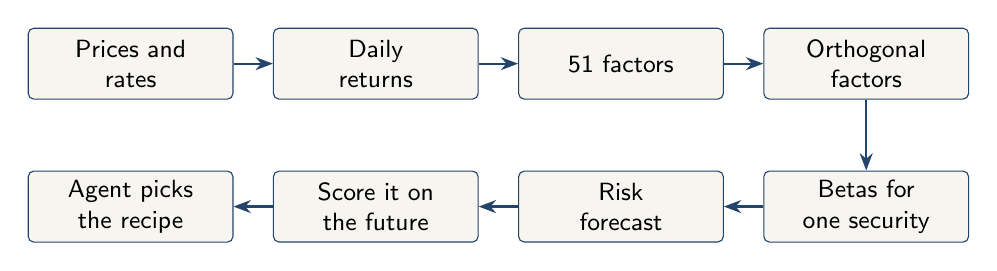
\begin{tikzpicture}[node distance=5mm,
  box/.style={draw=navy,fill=paper,rounded corners=2pt,minimum width=26mm,
              minimum height=9mm,font=\sffamily\small,align=center},
  arr/.style={-{Stealth[length=2.2mm]},draw=navy,thick}]
\node[box] (a) {Prices and\\rates};
\node[box,right=of a] (b) {Daily\\returns};
\node[box,right=of b] (c) {51 factors};
\node[box,right=of c] (d) {Orthogonal\\factors};
\node[box,below=9mm of d] (e) {Betas for\\one security};
\node[box,left=of e] (f) {Risk\\forecast};
\node[box,left=of f] (g) {Score it on\\the future};
\node[box,left=of g] (h) {Agent picks\\the recipe};
\draw[arr] (a)--(b); \draw[arr] (b)--(c); \draw[arr] (c)--(d);
\draw[arr] (d)--(e); \draw[arr] (e)--(f); \draw[arr] (f)--(g); \draw[arr] (g)--(h);
\end{tikzpicture}
\vfill
{\sffamily\small Companion to \texttt{factor-model-paper.pdf} and \texttt{model-agent.md}.
\\Every rule here is the rule the code applies; the file that applies it\\is named at the end of each recipe.\par}
\vspace{4mm}
{\sffamily\small October 2026\par}
\end{titlepage}

\tableofcontents
\clearpage

% =====================================================================
\section*{Before you start: how to read this book}
\addcontentsline{toc}{section}{Before you start}
\markboth{Before you start}{Before you start}

This book explains the whole model as a set of recipes. Each recipe says what
ingredients you need, what to do with them in order, and how to check the result.
Nothing in it needs a computer in principle: with a spreadsheet, a calculator and a
lot of patience you could rebuild every number the terminal shows. In practice the
code does it, and the last line of each recipe names the file that does.

The model answers one question:

\begin{center}
\emph{How much could this security's value move tomorrow, and over the next month,\\
and which kinds of market risk is that movement made of?}
\end{center}

It does this without looking inside the security. It never asks what a fund owns.
It only watches how the security's daily return moves together with a set of
\textbf{factors}: daily returns that each stand for one kind of market risk, such
as ``global stocks'', ``US interest rates'', ``the dollar'' or ``oil''. If a
security has gone up by about 1.2\% on days global stocks went up 1\%, it has a
\emph{loading} (a \emph{beta}) of about 1.2 on global stocks.

The work happens in seven stages, which are the seven parts of this book:

\begin{enumerate}[leftmargin=2.2em]
  \item \textbf{Prepare the ingredients}: turn raw prices and rates into clean daily returns on one calendar, in dollars, above cash.
  \item \textbf{Cook the factors}: build 40 core factors and 11 sector factors from those returns.
  \item \textbf{Separate the flavours}: strip from each factor what the factors above it already explain (orthogonalisation), and test that every factor is a well-behaved series.
  \item \textbf{Fit one security}: measure its betas on the factors, over a rolling window.
  \item \textbf{Forecast its risk}: combine the betas with the factors' own risk, add the part the factors cannot explain.
  \item \textbf{Taste the dish}: compare the forecast with what actually happened next.
  \item \textbf{Choose the recipe}: let the model agent try many variants and pick the simplest one that is as good as the best, then judge it once on data it never saw.
\end{enumerate}

A last part shows how the same forecast is applied to a portfolio.

\begin{tip}
Two rules run through every recipe. \textbf{Never use tomorrow's information
today}: every number dated $t$ is computed only from data known by the close of
day $t$. And \textbf{never invent data}: a value that is missing stays missing; it is
not filled in from the day before unless the gap is a short holiday.
\end{tip}

\subsubsection*{Notation used throughout}

\begin{tabularx}{\linewidth}{@{}lX@{}}
\toprule
$P_t$ & closing price on day $t$ (adjusted for dividends and splits) \\
$r_t$ & daily log return, $\ln(P_t/P_{t-1})$ \\
$c_t$ & cash rate on day $t$, the Federal Funds effective rate (FRED \texttt{DFF}), in percent per year \\
$f_t$ & a factor's return on day $t$ \\
$\beta$ & a loading: how much the security moves per unit move of a factor \\
$\Sigma$ & the covariance matrix of the factors: how much each moves, and how they move together \\
$\sigma$ & a volatility (standard deviation), quoted per year unless stated \\
252 & trading days in a year; a daily number times $\ann \approx 15.87$ gives an annual volatility \\
\bottomrule
\end{tabularx}

% =====================================================================
\section{Preparing the ingredients}

% ---------------------------------------------------------------------
\subsection{Stock the pantry}

\begin{ingredients}
\begin{itemize}[leftmargin=1.2em]
  \item Daily closing prices of about 250 exchange-traded funds and indices from Yahoo, with the \emph{adjusted} close (dividends reinvested).
  \item Daily interest rates from FRED: the cash rate \texttt{DFF}, US Treasury yields at 2, 5, 10 and 30 years, the 10-year breakeven inflation rate, SOFR, the effective funds rate, the VIX level, and policy rates for the euro, yen and franc.
  \item Euro-area and Japanese government yield curves (ECB, Bank of Japan, Ministry of Finance), from the warehouse.
  \item The weekly Chicago Fed financial conditions index (NFCI), \emph{as first published} and dated by the day it was published.
  \item For checking only: the Fama-French and AQR academic factors.
\end{itemize}
\end{ingredients}

\begin{method}
\begin{enumerate}[leftmargin=1.4em]
  \item Copy everything into one database. The warehouse tables are mirrored over a database link; Yahoo and FRED are downloaded fresh each night.
  \item For each fund, keep the adjusted close. Mark each series as \emph{total return} or \emph{price only}.
  \item Throw out, for factor building, every series that is price only: the \texttt{\^{}}-prefixed index levels carry no dividends.
  \item Throw out the \texttt{=F} futures series too: they are front-month prices glued together, with a fake jump at every roll.
\end{enumerate}
\end{method}

\begin{warn}
Using a price index (no dividends) for an equity factor makes every equity beta too
small by roughly the dividend yield. Using a stitched futures price for a commodity
factor adds a jump every month that no investor ever earned. Both give factors that
\emph{look} fine and are wrong, which is worse than having no factor.
\end{warn}

\doneby{\texttt{pipeline/sync.py}, \texttt{pipeline/ingest\_yahoo.py}, \texttt{pipeline/ingest\_fred.py}.}

% ---------------------------------------------------------------------
\subsection{Lay out the calendar}

All factors must live on the same list of days, or a ``252-day window'' would mean
different things for different factors.

\begin{method}
\begin{enumerate}[leftmargin=1.4em]
  \item Take every date on which any factor-input fund has a return.
  \item Remove Saturdays and Sundays. (Crypto trades at weekends; left in, it added 1,229 days on which nothing else traded.)
  \item Count, for each remaining date, how many factor-input funds reported. Find the largest count on any day.
  \item Keep a date only if at least 30\% of that largest count reported. This drops global holidays, when too few markets are open for a cross-asset factor to mean anything.
\end{enumerate}
The dates left are the \textbf{trading calendar}. Everything below is placed on it.
\end{method}

\doneby{\texttt{trading\_calendar} in \texttt{pipeline/build\_factors.py}.}

% ---------------------------------------------------------------------
\subsection{Turn prices into daily returns}

\begin{method}
For each fund and each trading day:
\[
  r_t = \ln\!\left(\frac{P_t}{P_{t-1}}\right)
\]
where $P$ is the adjusted close. Use logs, not simple percentage changes: log
returns add up over days, and converting currencies becomes a plain addition.
\end{method}

\begin{example}
A fund closes at 100.00 and then at 100.80. Its log return is
$\ln(100.80/100.00) = 0.00797$, i.e.\ 0.797\%. (The simple return is 0.800\%; for a
daily move the two are almost the same.)
\end{example}

% ---------------------------------------------------------------------
\subsection{Subtract the cash rate}

A factor should measure the reward for taking a risk, not the interest you would
have earned anyway. So every funded position has the day's cash rate taken off.

\begin{method}
\[
  r^{\text{excess}}_t = r_t - \frac{c_{t-1}/100}{252}
\]
Use \emph{yesterday's} cash rate: the overnight rate you earn on day $t$ was set on
day $t-1$. On a holiday with no rate printed, carry the last rate forward. (Here,
carrying forward is honest: an unchanged policy rate is a fact, not an invention.)
\end{method}

\begin{example}
The fund's log return is 0.797\% and yesterday's \texttt{DFF} was 5.33\%. A day's cash is
$0.0533/252 = 0.0212\%$. The excess return is $0.797\% - 0.021\% = 0.776\%$.
\end{example}

Two kinds of factor skip this step because no money is invested in them: a
\emph{long-short} spread (the cash earned on the short pays for the long) and a
\emph{currency index} like the dollar index.

% ---------------------------------------------------------------------
\subsection{Put everything in dollars}

All factors are in US dollars. A London fund priced in pounds has to be converted.

\begin{method}
\begin{enumerate}[leftmargin=1.4em]
  \item In logs, conversion is addition: $r^{\$}_t = r^{\text{local}}_t + r^{\text{FX}}_t$, where $r^{\text{FX}}$ is the log change in dollars per pound.
  \item Take the currency move \emph{at the New York close}, the same moment every other price is taken. Get it from the currency's New York-listed trust (e.g.\ \texttt{FXB} for the pound, \texttt{FXY} for the yen), not from Yahoo's \texttt{=X} rate, which since August 2010 is a day late.
  \item The trust earns a deposit rate minus a fee, which is not part of the exchange rate. Remove it: compute the trust's average daily drift over the spot rate across the past 252 days (ending yesterday) and subtract it from today's trust return.
  \[
    s_t = r^{\text{trust}}_t - a_t,\qquad
    a_t = \frac{\ln\frac{P_{t-1}}{P_{t-253}} - \ln\frac{S_{t-1}}{S_{t-253}}}{252}
  \]
  \item If the spot rate is missing for a few days, carry it at most 5 days. After that, the currency return is missing, and so is everything built on it.
\end{enumerate}
\end{method}

\begin{warn}
Carrying an exchange rate forward without limit makes a currency that ``stopped
moving'': every later change is exactly zero, and nothing downstream can tell that
from a quiet market.
\end{warn}

\doneby{\texttt{fx\_spot\_return} and \texttt{Panels.in\_base\_ccy} in \texttt{pipeline/build\_factors.py}.}

% =====================================================================
\section{Cooking the factors}

There are 51 factors: 40 core factors in nine blocks, and 11 sector factors that a
single stock may add for its own sector. They are built with a small number of
basic recipes. This part gives each basic recipe once; the table in
Recipe~\ref{rec:menu} then says which recipe and which ingredients make each factor.

Every factor has a \emph{level} in a hierarchy (0, 1, 2 or 3). Factors are cooked in
level order, lowest first, because in Part~\ref{part:orth} each factor is cleaned
against factors of lower level, which must therefore already exist.

% ---------------------------------------------------------------------
\subsection{The single-fund factor}\label{rec:single}

Most factors are simply one fund's excess return. This is how global equity
(\fid{eq\_global}, the MSCI ACWI fund), US investment-grade credit
(\fid{cr\_ig}, \texttt{LQD}) or gold (\fid{cm\_gold}, \texttt{GLD}) are made.

\begin{method}
\begin{enumerate}[leftmargin=1.4em]
  \item Take the fund's daily log return (Recipe 1.3).
  \item Subtract cash (Recipe 1.4), unless the fund is a currency index.
  \item If the fund is not priced in dollars, add the currency move (Recipe 1.5). Only the UK gilt fund \texttt{IGLT.L} needs this.
\end{enumerate}
\end{method}

% ---------------------------------------------------------------------
\subsection{The long-short spread}

Size (\fid{eq\_size}) is small companies minus large companies: the Russell 2000 fund
\texttt{IWM} minus the Russell 1000 fund \texttt{IWB}.

\begin{method}
$f_t = r^{\text{long}}_t - r^{\text{short}}_t$, using plain log returns. No cash is
subtracted: the two cash legs cancel.
\end{method}

% ---------------------------------------------------------------------
\subsection{The basket}

Cyclical-minus-defensive (\fid{eq\_cyclical}) is the average of five cyclical sector
funds (industrials, materials, energy, financials, consumer discretionary) minus
the average of three defensive ones (staples, utilities, health care).

\begin{method}
\[
  f_t = \frac{1}{n_L}\sum_{\text{long}} r_t \;-\; \frac{1}{n_S}\sum_{\text{short}} r_t
\]
Equal weights, plain log returns, no cash leg. The cross-asset risk-off factor
(\fid{liq\_risk\_off}) is made the same way: long Treasuries, the dollar and gold;
short high-yield bonds and emerging-market stocks.
\end{method}

% ---------------------------------------------------------------------
\subsection{A bond return from a yield}\label{rec:bond}

FRED gives yields, not prices. A yield going up is a bond price going down, so we
convert each day's yield change into the return of an imaginary bond bought at par
that day. This is a \emph{synthetic par bond}.

\begin{ingredients}
The yield $y$ of one maturity $T$ (in years) for today and yesterday, as a decimal;
yesterday's cash rate. Coupons are paid twice a year ($m=2$).
\end{ingredients}

\begin{method}
\begin{enumerate}[leftmargin=1.4em]
  \item Compute the bond's \textbf{duration} at \emph{yesterday's} yield. For a par bond:
  \[
    D = \frac{1-(1+y_{t-1}/m)^{-mT}}{y_{t-1}}
  \]
  Duration is how much the price falls, in percent, for a 1-point rise in yield.
  \item Compute its \textbf{convexity} $C$ at yesterday's yield (the small curvature correction; the formula is in \texttt{core/transforms.py}).
  \item Price the day:
  \[
    r_t = \underbrace{-D\,\Delta y_t}_{\text{price move}} \;+\;
          \underbrace{\tfrac12 C\,(\Delta y_t)^2}_{\text{curvature}} \;+\;
          \underbrace{\frac{y_{t-1} - c_{t-1}}{252}}_{\text{carry above cash}}
  \]
\end{enumerate}
\end{method}

\begin{example}
The 10-year yield rises from 4.00\% to 4.05\%, so $\Delta y = 0.0005$. At 4\% the
duration is $D = 8.18$ and the convexity $C = 78.9$. Cash was 4.33\%.
\begin{itemize}[leftmargin=1.2em]
\item price move: $-8.18 \times 0.0005 = -0.4088\%$
\item curvature: $\tfrac12 \times 78.9 \times 0.0005^2 = +0.0010\%$
\item carry: $(0.0400 - 0.0433)/252 = -0.0013\%$
\end{itemize}
The day's excess return is $-0.409\%$.
\end{example}

\begin{tip}
Duration and convexity are taken at \emph{yesterday's} yield. Taking them at today's
yield would use the very move being priced to decide how it is priced.
\end{tip}

% ---------------------------------------------------------------------
\subsection{Yield-curve portfolios: level, slope, curvature}

The curve factors (\fid{rt\_us\_level}, \fid{rt\_us\_slope}, \fid{rt\_us\_curve},
and the euro and Japanese level factors) are fixed-weight portfolios of synthetic
bonds.

\begin{method}
\begin{enumerate}[leftmargin=1.4em]
  \item Make the synthetic bond return (Recipe~\ref{rec:bond}) for each maturity needed. A missing yield may be carried at most 5 days (a local holiday), no further.
  \item Divide each bond's return by its own duration (at yesterday's yield). This makes a ``one-year-of-duration'' return $u^{(T)}$, so a 2-year and a 30-year bond can be compared like for like.
  \item Combine:
  \begin{itemize}[leftmargin=1.2em]
    \item \textbf{Level} (2, 5, 10, 30 years): the average of the four $u$'s.
    \item \textbf{Slope} (10s minus 2s): $u^{(10)} - u^{(2)}$, a steepener.
    \item \textbf{Curvature} (2, 5, 30 years): $2u^{(5)} - u^{(2)} - u^{(30)}$, long the middle, short the ends.
  \end{itemize}
  \item Multiply by 5 to scale back to the size of a 5-year-duration bond portfolio, a familiar magnitude.
\end{enumerate}
\end{method}

\begin{tip}
Fixed weights rather than principal components: the three factors mean the same
thing every day, their signs never flip, and no weight is fitted on future data.
Principal components are still computed on the Covariance page as a check that the
three span the same variance.
\end{tip}

\textbf{Breakeven inflation} (\fid{rt\_breakeven}) uses the same bond recipe on the
10-year breakeven rate, but with the carry removed completely: a breakeven is the
gap between two yields and pays no coupon of its own.

% ---------------------------------------------------------------------
\subsection{Currency factors}

\begin{method}
\begin{itemize}[leftmargin=1.2em]
  \item \textbf{Dollar} (\fid{fx\_usd}): the dollar index's log return, no cash leg.
  \item \textbf{Yen} (\fid{fx\_jpy}): the New York-close spot move of the yen against the dollar (Recipe 1.5). Positive means a stronger yen, the usual ``risk-off'' direction.
  \item \textbf{Emerging currencies} (\fid{fx\_em}): the excess return of the \texttt{CEW} fund.
  \item \textbf{Carry} (\fid{fx\_carry}): for each of the euro, yen and franc,
  \begin{enumerate}[leftmargin=1.4em]
    \item compute yesterday's rate gap: $g = (\text{foreign policy rate} - \text{US policy rate})/100/252$;
    \item hold the currency long if $g>0$, short if $g<0$;
    \item the leg's return is $\text{sign}(g)\times(\text{spot move} + g)$;
  \end{enumerate}
  then average the three legs.
\end{itemize}
\end{method}

\begin{warn}
The carry factor is an approximation. A real carry basket uses forward rates for
ten currencies; there are no forward points in the data, and only three non-dollar
policy rates. Treat a loading on it with suspicion.
\end{warn}

% ---------------------------------------------------------------------
\subsection{Factors from a rate or an index level: standardised changes}

Some useful series are not prices at all: the SOFR-minus-funds-rate spread, the
NFCI. Their units (basis points, index points) cannot be compared with returns.

\begin{method}
\textbf{Daily series} (SOFR minus EFFR, \fid{liq\_funding}):
\begin{enumerate}[leftmargin=1.4em]
  \item Take the daily change of the spread.
  \item Divide it by the standard deviation of the changes over the past 252 days (at least 60 needed). Now it is a ``z-score'': $+2$ means an unusually large widening.
  \item Rescale the whole series by one constant so that it has 10\% annual volatility, like a typical return factor: multiply by $\dfrac{0.10/\ann}{\text{sd of the series}}$.
\end{enumerate}
\end{method}

\begin{tip}
The constant in step 3 is a choice of units and nothing else. Multiplying a factor by
$k$ divides its beta by $k$ and multiplies its volatility by $k$, so every predicted
risk is unchanged. That is why it is safe to compute $k$ from the whole sample.
\end{tip}

\textbf{Weekly series} (NFCI, \fid{liq\_conditions}) get a different recipe, because
filling a weekly number into every day of the week would invent six days of
``information''.

\begin{method}
\begin{enumerate}[leftmargin=1.4em]
  \item Use each NFCI reading as first published, on the Wednesday it was published, not the Friday of the week it describes. If that Wednesday is a market holiday, move it to the next trading day.
  \item On a publication day, the factor is the change since the last reading, divided by the standard deviation of the past 52 changes (at least 12).
  \item On every other day, the factor is exactly \textbf{zero}.
  \item Rescale to 10\% annual volatility as above.
\end{enumerate}
\end{method}

\begin{warn}
Dated by its reference Friday, the NFCI ``knew'' five days early what equities did
that week: it correlated $-0.33$ with stock returns no one could yet have reacted to.
\end{warn}

% ---------------------------------------------------------------------
\subsection{Volatility factors}

\begin{method}
\begin{itemize}[leftmargin=1.2em]
  \item \textbf{Equity volatility} (\fid{vol\_equity}): the excess return of \texttt{VIXY}, a fund that holds VIX futures. A tradeable return, unlike the VIX level itself.
  \item \textbf{Variance risk premium} (\fid{vol\_variance\_premium}): what a seller of one day's variance earns:
  \[
    f_t = \frac{(\text{VIX}_{t-1}/100)^2}{252} - r_{t,\text{SPY}}^2
  \]
  i.e.\ yesterday's implied variance for one day, minus today's squared S\&P 500 return. Then rescale to 10\% volatility.
  \item \textbf{Rates volatility} (\fid{vol\_rates}): a ``surprise'' in the size of the Treasury fund \texttt{TLT}'s move:
  \begin{enumerate}[leftmargin=1.4em]
    \item keep a running exponentially weighted average of TLT's squared returns with a 21-day half-life; its square root at yesterday's close is yesterday's volatility forecast $s_{t-1}$;
    \item $f_t = |r_t|/s_{t-1} - 0.798$, where $0.798=\sqrt{2/\pi}$ is the average size of a normal surprise, so the factor averages zero when the forecast is right;
    \item rescale to 10\% volatility.
  \end{enumerate}
\end{itemize}
\end{method}

\begin{example}
VIX closed yesterday at 20. One day's implied variance is $0.20^2/252 = 0.000159$.
Today SPY moved 1\%, so realised variance is $0.01^2 = 0.000100$. The short-variance
seller earned $0.000059$ (before rescaling). On a 3\% day they would have lost
$0.000741$: the payoff is small most days and sharply negative on bad ones.
\end{example}

\begin{tip}
\fid{vol\_rates} used to be the daily change in a 21-day rolling volatility. Half of
that change was the squared return \emph{leaving} the window, three weeks after it
happened: an echo no security reacts to.
\end{tip}

% ---------------------------------------------------------------------
\subsection{Momentum strategies}

The two alternative-risk-premia factors are trading rules run over 13 funds: US,
developed and emerging stocks; long and medium Treasuries; commodities, gold, oil;
high-yield and investment-grade credit; the dollar, the euro and the yen.

\begin{method}
\textbf{Trend} (\fid{arp\_trend}), for day $t$:
\begin{enumerate}[leftmargin=1.4em]
  \item For each fund, add up its log returns over the past year but \emph{skip the latest month}: the 231 days ending 22 days ago. The sign of that sum is the signal ($+1$ up-trend, $-1$ down-trend).
  \item Compute its volatility over the 63 days ending yesterday.
  \item Position $=$ signal $/$ volatility, so quiet assets get bigger positions.
  \item The factor is $\sum(\text{position}\times\text{today's return}) / \sum|\text{position}|$.
\end{enumerate}
\textbf{Cross-sectional momentum} (\fid{arp\_xs\_momentum}):
\begin{enumerate}[leftmargin=1.4em]
  \item Compute the same skip-a-month trailing return for every fund, and rank them.
  \item Hold the top third long and the bottom third short, equally weighted within each.
  \item The factor is the average return of the longs minus that of the shorts.
\end{enumerate}
\end{method}

% ---------------------------------------------------------------------
\subsection{Sector factors}

\begin{method}
One factor per GICS sector, each the excess return of its SPDR sector fund
(\texttt{XLK} for technology, \texttt{XLF} for financials, and so on). They are
single-fund factors (Recipe~\ref{rec:single}). Two start late: real estate
(\texttt{XLRE}) in October 2015 and communication services (\texttt{XLC}) in June 2018.
\end{method}

They are not part of the forty. Adding eleven more columns to every regression would
cost more in noise than it explains. A stock may add the one factor of its own
sector, and only if the agent finds it earns its place (Part~\ref{part:agent}).

% ---------------------------------------------------------------------
\subsection{The full menu}\label{rec:menu}

The level column gives the cooking order; the last column says what each factor is
cleaned against in Part~\ref{part:orth}.

{\footnotesize
\begin{longtable}{@{}>{\ttfamily}l >{\raggedright\arraybackslash}p{1.9cm} >{\raggedright\arraybackslash}p{3.4cm} c >{\ttfamily\raggedright\arraybackslash}p{3.9cm}@{}}
\toprule
\textnormal{Factor} & Recipe & Made from & Lvl & \textnormal{Cleaned against} \\
\midrule
\endhead
\multicolumn{5}{@{}l}{\textit{Equity market}}\\
\fid{eq\_global} & single & ACWI & 0 & \textnormal{---} \\
\fid{eq\_us} & single & IVV & 1 & eq\_global \\
\fid{eq\_europe} & single & VGK & 1 & eq\_global \\
\fid{eq\_japan} & single & EWJ & 1 & eq\_global \\
\fid{eq\_em} & single & EEM & 1 & eq\_global \\
\fid{eq\_size} & spread & IWM $-$ IWB & 1 & eq\_global \\
\fid{eq\_cyclical} & basket & 5 cyclical $-$ 3 defensive sector funds & 1 & eq\_global \\
\multicolumn{5}{@{}l}{\textit{Equity style}}\\
\fid{sty\_value} & single & VLUE & 2 & eq\_global, eq\_us, eq\_cyclical \\
\fid{sty\_momentum} & single & MTUM & 2 & eq\_global, eq\_us, eq\_cyclical \\
\fid{sty\_quality} & single & QUAL & 2 & eq\_global, eq\_us, eq\_cyclical \\
\fid{sty\_lowvol} & single & USMV & 2 & eq\_global, eq\_us, eq\_cyclical \\
\multicolumn{5}{@{}l}{\textit{Rates}}\\
\fid{rt\_us\_level} & curve & US 2/5/10/30y & 0 & \textnormal{---} \\
\fid{rt\_us\_slope} & curve & US 10y $-$ 2y & 0 & \textnormal{---} \\
\fid{rt\_us\_curve} & curve & US 2/5/30y butterfly & 0 & \textnormal{---} \\
\fid{rt\_ea\_level} & curve & euro AAA 2/5/10/30y & 0 & rt\_us\_level \\
\fid{rt\_jp\_level} & curve & JGB 2/5/10/30y & 0 & rt\_us\_level \\
\fid{rt\_uk} & single, in \$ & IGLT.L & 0 & rt\_us\_level \\
\fid{rt\_breakeven} & bond, no carry & 10y breakeven & 0 & rt\_us\_level \\
\multicolumn{5}{@{}l}{\textit{Credit}}\\
\fid{cr\_ig} & single & LQD & 1 & rt\_us\_level, rt\_us\_slope \\
\fid{cr\_hy} & single & HYG & 1 & rt\_us\_level, rt\_us\_slope, eq\_global \\
\fid{cr\_loans} & single & BKLN & 1 & rt\_us\_level, cr\_hy \\
\fid{cr\_em\_hard} & single & EMB & 1 & rt\_us\_level, rt\_us\_slope, cr\_hy, eq\_global \\
\fid{cr\_em\_local} & single & EMLC & 2 & rt\_us\_level, cr\_em\_hard, fx\_usd \\
\multicolumn{5}{@{}l}{\textit{FX}}\\
\fid{fx\_usd} & single, no cash & dollar index & 0 & \textnormal{---} \\
\fid{fx\_jpy} & FX spot & yen via FXY & 1 & fx\_usd \\
\fid{fx\_em} & single & CEW & 1 & fx\_usd \\
\fid{fx\_carry} & carry & EUR, JPY, CHF rate gaps & 1 & fx\_usd, fx\_jpy \\
\multicolumn{5}{@{}l}{\textit{Commodities}}\\
\fid{cm\_broad} & single & DBC & 0 & \textnormal{---} \\
\fid{cm\_energy} & single & USO & 1 & cm\_broad \\
\fid{cm\_gold} & single & GLD & 1 & cm\_broad \\
\fid{cm\_industrial} & single & CPER & 1 & cm\_broad \\
\fid{cm\_agri} & single & DBA & 1 & cm\_broad \\
\multicolumn{5}{@{}l}{\textit{Volatility}}\\
\fid{vol\_equity} & single & VIXY & 1 & eq\_global \\
\fid{vol\_variance\_premium} & variance payoff & VIX, SPY & 1 & eq\_global \\
\fid{vol\_rates} & surprise & TLT & 1 & rt\_us\_level \\
\multicolumn{5}{@{}l}{\textit{Liquidity and stress}}\\
\fid{liq\_funding} & std.\ change & SOFR $-$ EFFR & 0 & \textnormal{---} \\
\fid{liq\_conditions} & release event & NFCI & 0 & \textnormal{---} \\
\fid{liq\_risk\_off} & basket & TLT, UUP, GLD $-$ HYG, EEM & 2 & eq\_global, rt\_us\_level, cr\_hy \\
\multicolumn{5}{@{}l}{\textit{Alternative risk premia}}\\
\fid{arp\_trend} & trend & 13 funds & 3 & eq\_global, rt\_us\_level, cm\_broad, fx\_usd \\
\fid{arp\_xs\_momentum} & ranking & 13 funds & 3 & eq\_global, arp\_trend \\
\multicolumn{5}{@{}l}{\textit{Sectors (role ``sector'', optional)}}\\
\fid{sec\_*} (11) & single & XLK, XLF, XLV, XLI, XLY, XLP, & 2 & eq\_global, eq\_us, eq\_cyclical \\
 & & XLE, XLB, XLU, XLRE, XLC & & \\
\bottomrule
\end{longtable}
}

\doneby{\texttt{pipeline/factor\_defs.py} (the menu) and \texttt{pipeline/build\_factors.py} (the cooking). Every formula is written out in full in \texttt{factor-formulas.md}.}

% =====================================================================
\section{Separating the flavours}\label{part:orth}

% ---------------------------------------------------------------------
\subsection{Orthogonalise down the hierarchy}

US stocks and global stocks move together almost perfectly (correlation 0.97).
Put both raw into one regression and the betas come out as large numbers of
opposite sign that mean nothing on their own. So each factor is cleaned of what
the factors above it already explain. What is left answers a sharper question:
\fid{eq\_us} becomes ``what US stocks did \emph{beyond} what global stocks did''.

\begin{ingredients}
The raw factor $f$ just cooked; the already-cleaned factors $X_1,\dots,X_k$ it is to be
cleaned against (last column of the menu).
\end{ingredients}

\begin{method}
Go through the factors in level order. For each factor with something to clean
against:
\begin{enumerate}[leftmargin=1.4em]
  \item Wait until 252 days of history exist. Before that the cleaned factor is missing: that is the price of not using the future.
  \item Every 21 trading days (about once a month), fit an ordinary least-squares regression of $f$ on $X_1..X_k$ with an intercept, using only the \textbf{504 trading days before today} (about two years) and only days where every series is present:
  \[
    f_s = a + b_1 X_{1,s} + \dots + b_k X_{k,s} + e_s
  \]
  \item For each of the next 21 days, the cleaned factor is what that fit does not explain:
  \[
    f^{\perp}_t = f_t - a - b_1 X_{1,t} - \dots - b_k X_{k,t}
  \]
  \item Store both versions: the raw one (\texttt{ret\_excess}) and the cleaned one (\texttt{ret\_orth}).
  \item When a later factor is cleaned against this one, use the \emph{cleaned} version. The hierarchy compounds: credit is cleaned against cleaned rates, style against cleaned equity, and so on.
\end{enumerate}
Factors with nothing in their last column are left as they are.
\end{method}

\begin{example}
On the last refit, regressing \texttt{IVV}'s excess return on \fid{eq\_global} over the
previous 504 days gave $a = 0.0001$ and $b = 0.95$. Today IVV returned 1.00\% and
global equity 0.80\%. The cleaned US factor is
$0.0100 - 0.0001 - 0.95\times0.0080 = 0.0023$, i.e.\ 0.23\%: US stocks beat what
the global market alone would have predicted by about a quarter of a percent.
\end{example}

\begin{tip}
Why a trailing two-year window, refitted monthly? Fitting once on the whole history
would make the cleaned factors exactly uncorrelated, but would put 2026 information
into 2008 values, flattering the model exactly where it is judged. A window that
grows forever never forgets 2008, so its betas stay wrong for a decade. The trailing
window leaves a small leftover correlation ($-0.05$ for emerging against global
equity) and uses no future data. The leftover is not lost: the factor covariance in
Part~\ref{part:risk} measures it.
\end{tip}

\begin{warn}
The cleaned factor is not what the factor \emph{earned}. \fid{eq\_us} earns about 13\%
a year at 17\% volatility; its cleaned version earns about $-0.2\%$ at 4\%. That is
why the terminal has a Factor Explorer (cleaned, what the model uses) and a separate
Raw Explorer (raw, what the market did).
\end{warn}

\doneby{\texttt{core/orthogonalize.py} (\texttt{residualize\_rolling}), called from \texttt{pipeline/build\_factors.py}.}

% ---------------------------------------------------------------------
\subsection{Check that the style factors are what they say}

The style factors are long-only funds, not the academic long-short portfolios. Check
them against the published Fama-French and AQR factors, which arrive one to two
months late and can never drive a daily model, but are good for checking.

\begin{method}
Correlate each cleaned factor with its academic counterpart over the days both exist.
\end{method}

\begin{center}
\small
\begin{tabular}{@{}llccc@{}}
\toprule
Factor & Reference & Raw & Cleaned & Days \\
\midrule
\fid{eq\_global} & Mkt-RF & 0.963 & 0.963 & 4{,}551 \\
\fid{eq\_size} & SMB & 0.914 & 0.874 & 4{,}287 \\
\fid{sty\_momentum} & Mom & 0.207 & 0.638 & 3{,}006 \\
\fid{sty\_value} & HML & 0.194 & 0.499 & 3{,}006 \\
\fid{sty\_lowvol} & BAB & $-$0.002 & 0.199 & 3{,}363 \\
\fid{sty\_quality} & RMW & $-$0.145 & 0.143 & 2{,}943 \\
\bottomrule
\end{tabular}
\end{center}

Raw, the style funds barely resemble their targets, because market moves swamp the
style. Cleaned, momentum and value become recognisable. Quality and low volatility
remain weak: they are kept so the block is complete, not because they are good.

% ---------------------------------------------------------------------
\subsection{Taste every factor: the stationarity battery}

A factor must be a well-behaved return series: no trend in its level, no stale
prices, no hidden break. Test this rather than assume it.

\begin{method}
For each factor, on its full history and on the last 252 days, run:
\begin{center}
\small
\begin{tabularx}{\linewidth}{@{}lXl@{}}
\toprule
Test & What it catches & Effect \\
\midrule
ADF and KPSS, read together & a level that should have been a change & can block \\
Zivot-Andrews & a one-off break that looks like a trend & warning \\
Variance ratio & stale or smoothed prices & warning \\
Ljung-Box & day-to-day autocorrelation & warning \\
Share of zero returns & a series that is not really trading & warning, or fail above 50\% \\
ARCH-LM & calm and stormy spells & recorded only \\
\bottomrule
\end{tabularx}
\end{center}
Read ADF and KPSS as a pair, at 5\%. ADF assumes ``trending'' and tries to reject it;
KPSS assumes ``steady'' and tries to reject that. So:
\begin{itemize}[leftmargin=1.2em]
  \item ADF rejects, KPSS does not $\Rightarrow$ \textbf{stationary}, fine;
  \item KPSS rejects, ADF does not $\Rightarrow$ \textbf{unit root}: the series blocks;
  \item both reject $\Rightarrow$ probably a break or changing volatility: warning;
  \item neither rejects $\Rightarrow$ inconclusive: warning.
\end{itemize}
\end{method}

\begin{tip}
Calm and stormy spells (ARCH effects) are \emph{recorded but never block}. A series
whose volatility clusters is still stationary, and almost every financial series
clusters. What clustering tells you is to use robust standard errors and a
fast-moving covariance, not to throw out the factor.
\end{tip}

\doneby{\texttt{core/stationarity.py}, \texttt{pipeline/run\_diagnostics.py}.}

% =====================================================================
\section{Fitting one security}\label{part:fit}

% ---------------------------------------------------------------------
\subsection{Prepare the security}

\begin{method}
\begin{enumerate}[leftmargin=1.4em]
  \item Pull its daily prices. Make log returns (Recipe 1.3), subtract cash (Recipe 1.4), and if it is not in dollars convert at the New York close (Recipe 1.5).
  \item Run the stationarity battery on its returns.
  \item Note its asset class (equity, Japanese equity, fixed income, commodity, FX), its GICS sector if it is a stock, and whether it closes before New York (a Tokyo stock does).
\end{enumerate}
\end{method}

% ---------------------------------------------------------------------
\subsection{Choose the factors}

\begin{method}
Pick one of:
\begin{itemize}[leftmargin=1.2em]
  \item \textbf{All} forty core factors.
  \item The \textbf{template} for the asset class: its own blocks plus a handful of cross-asset factors. For a US stock that is the equity and style blocks plus US level and slope, high yield, the dollar, broad commodities, energy, equity volatility and risk-off. Fixed income gets rates and credit plus global equity, the dollar, rates volatility, risk-off and financial conditions; and so on.
  \item Optionally, for a stock, add the factor of its own sector.
\end{itemize}
Choose also the \textbf{panel}: cleaned factors (the default, and the better forecaster) or raw factors (easier to explain: a beta of 1.02 to global equity means what it says).
\end{method}

\begin{tip}
Fewer factors means less noise. With forty factors on 252 days, the random error in
the betas alone adds about $k/n = 40/252 \approx 16\%$ to the unexplained variance.
A template keeps the factors that can plausibly matter.
\end{tip}

% ---------------------------------------------------------------------
\subsection{Run the rolling regression}

\begin{ingredients}
The security's excess return $y$; the chosen factors' returns; a set of settings:
window length (126 to 756 days), step (fixed at 21 days for the agent),
estimator, weighting, Dimson lags, winsorising.
\end{ingredients}

\begin{method}
Every 21 trading days (the \emph{step}), on the date $t$ that ends a window:
\begin{enumerate}[leftmargin=1.4em]
  \item Take the last $n$ days up to and including $t$ (e.g.\ $n=252$). Keep only factors with enough data in the window; drop the rest for this window.
  \item Optionally \textbf{winsorise}: clip each series at its 1st and 99th percentile within the window, so one bad print cannot dominate.
  \item Fit
  \[
    y_s = \alpha + \beta_1 f_{1,s} + \dots + \beta_k f_{k,s} + \varepsilon_s
    \qquad (s = t-n+1, \dots, t)
  \]
  with one of
  \begin{itemize}[leftmargin=1.2em]
    \item \textbf{OLS}: ordinary least squares, every day weighted equally;
    \item \textbf{Huber}: like OLS but days with very large residuals get less weight (5 re-weighting passes, tuning constant 1.345), so one wild day pulls less;
    \item \textbf{Ridge}: OLS plus a penalty $\lambda$ that pulls betas towards zero, which steadies them when factors overlap.
  \end{itemize}
  Optionally weight recent days more (EWMA weighting with a half-life of 42 to 252 days).
  \item For a security that closes before New York, add \textbf{Dimson lags}: also regress on \emph{yesterday's} (and the day before's) US-hours factors, because a Tokyo stock reacts to New York's move only the next morning. The total beta is the sum of the lags.
  \item Record the betas, their full covariance $V$ (robust Newey-West ``HAC'' errors), $R^2$, residual volatility, the condition number of the standardised factors, the largest variance inflation factor (VIF), and residual tests.
  \item Record how much the beta vector changed since the last window (L1 distance and correlation, on the factors both windows share): a sudden jump is a drift alert.
\end{enumerate}
The betas estimated at $t$ are \emph{in force} from $t$ until the next window, 21 days later.
\end{method}

\begin{warn}
A window where few factors yet existed can be nearly singular: the factors are
almost linear combinations of each other and the betas explode. Once that produced a
360\% predicted volatility for Apple. So a window is flagged \emph{ill-conditioned}
when the condition number (on standardised factors) exceeds 200, or, on the cleaned
panel only, when the largest VIF exceeds 100. Flagged windows are stored but never
scored. (On the raw panel high VIFs are what the factor set is by design, so the VIF
rule does not apply there.)
\end{warn}

\doneby{\texttt{core/regression.py}, \texttt{pipeline/run\_estimation.py}.}

% =====================================================================
\section{Forecasting the risk}\label{part:risk}

The risk of a security is split in two: the part that comes from the factors
(\emph{systematic}), and the part that is its own (\emph{specific}).
\[
  \sigma^2_{\text{total}} \;=\; \underbrace{\beta^{\top}\Sigma_F\,\beta}_{\text{systematic}}
  \;+\; \underbrace{\sigma^2_{\varepsilon}}_{\text{specific}}
\]

% ---------------------------------------------------------------------
\subsection{Estimate the factor covariance}

\begin{ingredients}
Daily returns of the factors the betas refer to, \emph{from the same panel}
(cleaned betas need the covariance of cleaned factors), for a trailing window
(252, 504 or 756 days) ending on the forecast date.
\end{ingredients}

\begin{method}
Choose one estimator:
\begin{itemize}[leftmargin=1.2em]
  \item \textbf{Sample}: the ordinary covariance, every day equal.
  \item \textbf{EWMA}: recent days count more; a day $j$ days old has weight $0.5^{\,j/h}$ for half-life $h$ (5 to 126 days). Short half-lives follow volatility quickly.
  \item \textbf{Ledoit-Wolf}: the sample covariance pulled part of the way towards a simple target in which every pair of factors has the same correlation. Steadier, especially when there are many factors and few days.
  \item \textbf{Blend}: $a\times$EWMA $+\,(1-a)\times$Ledoit-Wolf. The original model used $a = 0.6$ with a 60-day half-life.
\end{itemize}
Annualise (times 252). Check that the matrix is valid (no negative eigenvalues). If
it is not, set the negative eigenvalues to a tiny positive number and then rescale so
each factor's volatility is exactly what it was before.
\end{method}

% ---------------------------------------------------------------------
\subsection{Systematic risk, with the noise taken out}

\begin{method}
\begin{enumerate}[leftmargin=1.4em]
  \item Take the betas in force on the forecast date and compute $\beta^{\top}\Sigma_F\beta$.
  \item Optionally \textbf{debias}: subtract $\operatorname{tr}(\Sigma_F V)$, where $V$ is the betas' covariance from the regression. Estimated betas are noisy, and noise always \emph{adds} to $\beta^{\top}\Sigma\beta$ on average. This term is that addition.
\end{enumerate}
\end{method}

% ---------------------------------------------------------------------
\subsection{Specific risk}

\begin{method}
Choose one:
\begin{itemize}[leftmargin=1.2em]
  \item \textbf{In-sample}: the residual volatility of the regression window.
  \item \textbf{Out-of-sample}: each day, take the security's return minus what the betas in force predicted. Square it, subtract the beta-noise part $f^{\top}Vf$ (so it is not counted twice), and keep an exponentially weighted average (half-life 21, 63 or 126 days).
\end{itemize}
Never let specific volatility fall below \textbf{2\% a year}. The floor is the model
admitting it cannot see every risk.
\end{method}

% ---------------------------------------------------------------------
\subsection{Put the forecast together}

\begin{method}
\begin{enumerate}[leftmargin=1.4em]
  \item Total variance $=$ systematic $+$ specific. Its square root is the annual volatility forecast; divide by $\ann$ for a day.
  \item \textbf{Refresh}: either keep the forecast fixed until the next regression window (monthly), or recompute the covariance and specific risk every day while holding the betas. Daily refresh follows volatility far better.
  \item \textbf{Value at Risk}: the 95\% one-day VaR is $z_{0.95}\times$ daily volatility, with $z = 1.645$ for a normal distribution (2.326 at 99\%). Or use a Student $t$ whose fatness is fitted to the security's own past returns divided by their own EWMA volatility, which gives larger tails.
\end{enumerate}
\end{method}

\begin{example}
A stock has betas 1.1 on global equity and 0.3 on a style factor. Global equity has
16\% volatility, the style factor 8\%, correlation 0.2. Specific volatility is 20\%.
\begin{itemize}[leftmargin=1.2em]
  \item systematic: $1.1^2(0.16^2) + 0.3^2(0.08^2) + 2(1.1)(0.3)(0.2)(0.16)(0.08) = 0.0332$
  \item specific: $0.20^2 = 0.0400$
  \item total: $0.0732$, so volatility $=\sqrt{0.0732} = 27.1\%$ a year, $27.1/15.87 = 1.70\%$ a day
  \item 95\% one-day VaR (normal) $= 1.645\times1.70\% = 2.80\%$
\end{itemize}
Systematic risk is 45\% of the total; the rest is the stock's own.
\end{example}

% ---------------------------------------------------------------------
\subsection{The one-month forecast}

A month's risk is not simply a day's risk times $\sqrt{21}$, for two reasons.

\textbf{Markets close at different times.} The euro and Japanese curves, a London
fund and the FX fixes close before New York, so one day's shock lands in two days'
returns. A daily covariance cannot see this; a 21-day return contains it.

\begin{method}
Add the lead-lag term: with $\Gamma_l$ the covariance of factors today with factors $l$
days earlier, the $h$-day variance per day is
\[
  \Gamma_0 + \sum_{l=1}^{L}\Bigl(1-\frac{l}{h}\Bigr)\bigl(\Gamma_l + \Gamma_l^{\top}\bigr)
\]
with $L$ = 0, 1, 2, 3 or 5 lags (zero unless the evidence is clear). For a Dimson model,
use the summed beta here.
\end{method}

\textbf{Volatility reverts.} After a shock it falls; after a calm spell it rises. A
forecast made today should drift towards the long-run level over the month.

\begin{method}
With half-life $H$ (126, 63 or 21 days, or none), $\varphi = 0.5^{1/H}$ and horizon $h$:
\[
  \text{month forecast} = LR + g\,(\text{today} - LR),\qquad
  g = \frac{1-\varphi^{h}}{h(1-\varphi)}
\]
$LR$ is the long-run level: the Ledoit-Wolf covariance of the same window, and the
in-sample specific variance. For a day ahead $g = 1$, so the daily forecast is untouched.
\end{method}

\begin{example}
With $H = 63$ and $h = 21$: $\varphi = 0.98906$ and $g = 0.898$. If today's variance
is twice the long-run level, the month forecast is $LR + 0.898\,LR = 1.90\times LR$:
the shock is expected to fade a little within the month.
\end{example}

\doneby{\texttt{core/covariance.py}, \texttt{pipeline/run\_risk.py}.}

% =====================================================================
\section{Tasting the dish: scoring the forecast}\label{part:score}

A forecast is only worth something if it is right about the future. So every
forecast dated $t$ is compared with what happened on days $t+1$ to $t+h$. The
betas come from a window ending at or before $t$, the covariance from returns up to
$t$: the gap is built in, not a convention.

\begin{method}
Collect all forecasts with their outcomes, excluding ill-conditioned windows, and compute:
\begin{enumerate}[leftmargin=1.4em]
  \item \textbf{Bias statistic}. Divide each return by the volatility forecast in force for it: $z = r/\hat\sigma$. The standard deviation of the $z$'s should be 1. Above 1: risk was under-forecast. Below 1: over-forecast. With $n$ forecasts, anything within $1\pm\sqrt{2/n}$ is acceptable.
  \item \textbf{Mincer-Zarnowitz}. Regress realised variance on forecast variance: realised $= a + b\times$forecast. A good forecast has $a=0$, $b=1$; test both together.
  \item \textbf{Kupiec}. Count the days the loss exceeded the VaR. At 95\% you expect 5\% of days. Is the count too far from that?
  \item \textbf{Christoffersen}. Are the breaches independent, or do they come in bunches? A model can have exactly the right count, all in one week.
  \item \textbf{Against a naive forecast}. Score the model, the security's own EWMA volatility and a one-factor market model with the QLIKE loss,
  \[
    \text{QLIKE} = \frac{\text{realised}^2}{\text{forecast}^2} - \ln\frac{\text{realised}^2}{\text{forecast}^2} - 1,
  \]
  which is zero for a perfect forecast and ranks variance forecasts fairly even when ``realised'' is noisy. Compare with a Diebold-Mariano test. A model that is significantly \emph{worse} than the security's own past volatility has not earned its factors.
\end{enumerate}
\end{method}

\begin{warn}
A Mincer-Zarnowitz slope below 1 is partly unavoidable. Realised volatility over the
next 21 days mixes calm and stormy days, while the forecast refers to one moment. In
a simulation with a \emph{perfect} forecast, regimes lasting 21 days gave a slope of
0.50. So a low slope is not by itself proof the model over-reacts.
\end{warn}

\doneby{\texttt{core/risk.py}.}

% =====================================================================
\section{Choosing the recipe: the model agent}\label{part:agent}

Parts 4 and 5 left many choices open: which factors, which window, which estimator,
which covariance, how often to refresh. None is right for every security. The
agent tries many combinations for one security and picks one. A language model
(DeepSeek) suggests what to try next; \emph{every number is computed by the code},
and the language model never fits, scores, picks the winner or writes the verdict.

% ---------------------------------------------------------------------
\subsection{Lock away the test data}

\begin{method}
\begin{enumerate}[leftmargin=1.4em]
  \item Lay a monthly grid of forecast dates (every 21 trading days) over the security's history.
  \item The last 36 grid dates (or 30\% of the grid if that is fewer, never fewer than 24) are the \textbf{test span}. Put them in a locked drawer.
  \item Everything before is the \textbf{validation span}, less an \emph{embargo}: drop validation dates whose 21-day outcome would reach into the test span.
  \item During the search, the code literally hands the scoring routine a copy of the data that ends the day before the test span. Nothing can peek.
\end{enumerate}
\end{method}

\begin{tip}
Try forty recipes and keep the one that scored best, and you have found the luckiest,
not the best. Its score is flattered by the search. The only honest score is one on
data the search never touched, taken once. A test runs the whole agent twice, once
with every test-span return multiplied by fifty, and checks the choice is identical.
\end{tip}

% ---------------------------------------------------------------------
\subsection{Gather the candidates}

Each candidate is one full recipe: the fitting half (panel, factors, window,
weighting, estimator, Dimson lags, winsorising, sector) and the risk half
(covariance method, half-life, blend weight, window; specific risk; debiasing;
refresh; VaR distribution).

\begin{method}
\begin{enumerate}[leftmargin=1.4em]
  \item \textbf{Seed} with fixed starting points: the original model (cleaned panel, all factors, 252-day OLS, 60/40 blend, held for a month); the raw panel; ridge; a longer decayed window; a fast, daily-refreshed, debiased forecast with $t$-VaR; the asset-class template; one Dimson lag for an early-closing security; the template with its own sector for a stock.
  \item \textbf{Pool}: add up to eight recipes that won or nearly won in earlier runs, for this security or similar ones. Only the recipes travel, never their scores.
  \item \textbf{Score} each candidate on the validation span: run Parts 4 and 5, and compute the daily QLIKE of the forecast in force each day (scored against that day's squared return).
  \item \textbf{Propose more}. The language model sees the profile, every candidate's validation numbers and the critic's hints, and replies with up to six new candidates, or ``stop''. The \emph{critic} is a set of plain rules that read the leader's diagnostics: ``loses to own EWMA, so the forecast is too slow; try a shorter half-life''; ``99\% breaches far too many while 95\% is fine, so the tails are too thin; try $t$-VaR''. If the language model fails twice, the critic proposes instead.
  \item Repeat steps 3 and 4 for at most five rounds, forty candidates or thirty minutes.
\end{enumerate}
\end{method}

% ---------------------------------------------------------------------
\subsection{Pick the winner}

\begin{method}
\begin{enumerate}[leftmargin=1.4em]
  \item \textbf{Model confidence set}. Find every candidate that cannot be told apart from the best at 90\% confidence (Hansen-Lunde-Nason, with a block bootstrap of the daily loss). The rest are significantly worse and drop out.
  \item \textbf{Calibration screen}. Within the set, keep only candidates whose validation forecasts were calibrated: bias statistic within $1\pm\sqrt{2/n}$ and Kupiec not rejected at 95\% or 99\%. (If none pass, keep the set.)
  \item \textbf{Simplest wins}. Among those left, pick the one with the fewest effective parameters (the number of factors; for ridge, fewer because the betas are shrunk). Break ties on the loss. The stock's own sector factor is not counted as a parameter: its value lies in what stocks of one sector share, which one stock's loss cannot see.
  \item \textbf{Fix the month forecast}. With the winner chosen, try 0, 1, 2, 3 and 5 lead-lag lags, then mean reversion of none, 126, 63 and 21 days, on the validation span's 21-day returns. Keep the simplest whose loss is within one standard error of the best.
\end{enumerate}
\end{method}

% ---------------------------------------------------------------------
\subsection{Open the drawer once: the verdict}

\begin{method}
Run the chosen recipe on the test span and check each gate:
\begin{center}
\small
\begin{tabularx}{\linewidth}{@{}lX@{}}
\toprule
Gate & Rule \\
\midrule
\multicolumn{2}{@{}l}{\textit{Correctness: any failure is a fail}}\\
test sample & at least 24 test forecasts, else ``insufficient data'' \\
forecasts issued & a forecast on at least 95\% of test dates \\
conditioning & at most 10\% of test windows ill-conditioned \\
stationary & the security's returns do not fail the battery \\
\multicolumn{2}{@{}l}{\textit{Value: failure on the monthly loss is a fail}}\\
beats naive & not significantly worse than own EWMA on monthly QLIKE ($p<0.05$) \\
\ldots day by day & the same on the daily loss; losing is a caveat \\
\multicolumn{2}{@{}l}{\textit{Calibration: each failure is a caveat}}\\
bias & 21-day bias statistic within $1\pm\sqrt{2/n}$ \\
Mincer-Zarnowitz & $a=0$, $b=1$ not rejected \\
VaR count & Kupiec not rejected at 95\% and at 99\% \\
VaR clustering & Christoffersen not rejected at 95\% \\
circularity & the security is not itself an input to one of its factors \\
\bottomrule
\end{tabularx}
\end{center}
No caveats: \textbf{pass}. One or two: \textbf{pass with caveats}. More: \textbf{fail}.
\end{method}

The chosen recipe, its betas, forecasts and both backtests (full history and test
span only) are stored, so every page of the terminal reads it like any other model.
Forecasts dated before the test span are marked \emph{in selection sample}: they
include the dates the recipe was chosen on, and are not evidence for it.

\doneby{\texttt{agent/graph.py} (the workflow), \texttt{agent/space.py}, \texttt{agent/evaluate.py}, \texttt{agent/critic.py}, \texttt{agent/llm.py}, \texttt{core/selection.py}.}

% =====================================================================
\section{Serving a portfolio}

\begin{ingredients}
Weights $w_i$ for each holding; each holding's betas $\beta_i$ (a 252-day OLS refitted
every 21 days on the cleaned factors, its asset-class template, plus its own sector
factor for a stock or a sector fund), beta covariances $V_i$ and specific variances.
\end{ingredients}

\begin{method}
\begin{enumerate}[leftmargin=1.4em]
  \item Add up the exposures: $x = \sum_i w_i\beta_i$ (the portfolio's beta on each factor).
  \item Estimate the factor covariance as a mix of three speeds: 80\% a 5-day EWMA, 10\% a 63-day EWMA, 10\% a 252-day EWMA. It reacts within days without collapsing in one quiet week.
  \item Next-day variance:
  \[
    \hat\sigma^2_p = x^{\top}\Sigma_F x \;-\; \sum_i w_i^2\operatorname{tr}(\Sigma_F V_i) \;+\; \sum_i w_i^2\hat\sigma^2_{\varepsilon,i}
  \]
  Specific risks add with squared weights: they are assumed unrelated across holdings, which is why stocks need their sector factor (it moves the shared sector part out of ``specific'').
  \item For the month, revert towards the 252-day level with a 63-day half-life (Recipe 5.5).
  \item Split the risk by \textbf{Euler contributions}: each holding's (or factor block's) share is its weight times how much the total would change per unit more of it. The shares add up to 100\%.
  \item Against a benchmark, run the same recipe on the \emph{active} weights (portfolio minus benchmark) to get the tracking error.
\end{enumerate}
\end{method}

\begin{warn}
A fund that is itself an input to a factor (say \texttt{HYG}, which \emph{is} the
high-yield factor) has loadings that just restate the factor's recipe. Its risk still
adds up correctly, but its betas explain nothing. The terminal flags it.
\end{warn}

\doneby{\texttt{pipeline/portfolio\_risk.py}, \texttt{core/portfolio.py}, \texttt{pipeline/run\_portfolio.py} (the 54-stock validation).}

% =====================================================================
\appendix
\renewcommand{\thesection}{\Alph{section}}
\titleformat{\section}{\sffamily\Large\bfseries\color{navy}}{Appendix \thesection}{0.8em}{}

\section{Letting the machine cook}

Everything above, in the order a fresh install runs it:

\begin{code}
python -m backend.pipeline.apply\_schema       \# create the database\\
python -m backend.pipeline.sync -{}-full        \# Part 1: warehouse data\\
python -m backend.pipeline.ingest\_yahoo -{}-full\# Part 1: prices\\
python -m backend.pipeline.ingest\_fred -{}-full \# Part 1: rates\\
python -m backend.pipeline.build\_factors      \# Parts 2-3: factors, cleaned\\
python -m backend.pipeline.run\_diagnostics    \# Part 3: stationarity battery\\
python -m backend.pipeline.sync -{}-security US:AAPL\\
python -m backend.agent.run -{}-instrument US:AAPL  \# Parts 4-7\\
python -m backend.pipeline.run\_portfolio      \# Part 8: 54-stock check
\end{code}

Or, for a hand-set recipe instead of the agent's:

\begin{code}
python -m backend.pipeline.run\_estimation -{}-instrument US:AAPL -{}-window 252 -{}-step 1m\\
python -m backend.pipeline.run\_risk -{}-instrument US:AAPL -{}-horizon 21
\end{code}

\section{Kitchen glossary}

\begin{tabularx}{\linewidth}{@{}lX@{}}
\toprule
Beta (loading) & how much a security moves per unit move of a factor \\
Cleaned factor & a factor with what the higher-level factors explain removed (orthogonalised) \\
Condition number & how close the factors in a window are to repeating each other; large means unstable betas \\
Covariance & how much two series move together; on the diagonal, each one's variance \\
Dimson lag & regressing on yesterday's factors too, for a market that closes earlier \\
EWMA & exponentially weighted moving average: recent days count more, halving every half-life \\
Excess return & return minus what cash would have paid \\
Half-life & the age at which a day's weight has halved \\
HAC errors & standard errors that allow for autocorrelation and changing volatility \\
Ledoit-Wolf & a covariance pulled towards a simple target to reduce noise \\
QLIKE & a score for a variance forecast; zero is perfect, lower is better \\
Specific risk & the part of a security's risk the factors do not explain \\
Stationary & a series whose behaviour does not drift over time \\
Test span & the last stretch of history, kept unseen until the recipe is chosen \\
VaR & Value at Risk: a loss exceeded on only 5\% (or 1\%) of days \\
VIF & variance inflation factor: how much one factor is explained by the others \\
Winsorise & clip extreme values at chosen percentiles \\
\bottomrule
\end{tabularx}

\end{document}
